\section{Grundvoraussetzungen} \label{chap:3}
\subsection{Installation}
\LaTeX\ ist kein eigenständiges Programm, sondern baut auf dem Textsatzsystem \TeX\ auf, wobei viele \TeX\ Distributionen \LaTeX\ schon beinhalten. Beide Teile sind kostenlos verfügbar.
Online Services wie Overleaf, Paaperia, Datazar, und \LaTeX\ base bieten einfach zu verwendende, kollaborative Web-Varianten, welche keine Installation auf dem eigenen Computer vorraussetzen.
TeX-Distributionen für verschiedene Betriebsysteme und Verlinkungen zu Online-Varianten sind unter folgendem Link zu finden: \url{www.latex-project.org/get}

\subsection{Dokumentstruktur}
Jedes Dokument benötigt eine bestimmte Grundordnung. 	
"Wenn ein unordentlicher Schreibtisch einen unordentlichen Geist repräsentiert, was sagt dann ein leerer Schreibtisch über den Menschen, der ihn benutzt aus?" \cite{albertzitat}
Man kann den grundsätzlichen Aufbau eines Dokuments in Präambel und Dokumentenkörper aufteilen. Die Präambel enthält Definitionen, welche für das ganze Dokument geltend sind. Der Dokumentenkörper beschreibt grob alles, was sich zwischen \texttt{\textbackslash begin\{document\}} und \texttt{\textbackslash end\{document\}} befindet und ist typischerweise unter den Definitionen der Präambel positioniert.
\cite[vgl.][S.19f]{Vosz2018}\\\\
Ein Kommentiertes Beispiel zur Dokumentenstruktur befindet sich im Listing \ref{lst:dokumentenstruktur}. Der Output ist in Abbildung \ref{fig:dokumentenstruktur} zu sehen.

\begin{listing}[H]
    \caption[Dokumentenstruktur]{Kommentiertes Beispiel zur Dokumentenstruktur in \LaTeX\ }
    \begin{minted}
    [
    firstnumber=1,
    frame=lines,
    framesep=2mm,
    baselinestretch=1.2,
    linenos
    ]
{Tex} 
\documentclass[a5paper,10pt,english,ngerman]{scrartcl} 
%Papiergröße: a5
%Schriftgröße: 10pt
%Sprachen: Deutsch(Hauptsprache, da zuletzt definiert), Englisch
%KOMA-Script-Klasse: scrartcl

\usepackage{babel} 
%Sprachpaket: babel
\usepackage[T1]{fontenc} 
%Paket für Schriftkodierung, unter LuaLaTeX: %\usepackage{fontspec}
\usepackage[utf8]{inputenc} %Encoding: UTF8
%Die LaTeX/TeX engine ist standardmäßig auf ASCII ausgerichtet.
\usepackage{mathptmx} 
%Schriftpaket: Times

\title{Wissenschaftliche Textverarbeitung mit \LaTeX}
\author{Max Mustermeyer}
\date{\today}
%Definieren Titel, Autor, Datum

\begin{document}
%Beginn des Dokumentenkörpers

\maketitle
%Formatierte Ausgabe von \title, \author, und \date

\begin{abstract}
%Zusammenfassung (Englisch)
This document serves as an example for a basic structure in \LaTeX.
\end{abstract}

\section{Einführung}
%Abschnitt mit der Überschrift "Einführung"
\LaTeX\ ist die Abkürzung für Lamport \TeX, benannt
nach ihrem Entwickler Leslie Lamport.

\end{document}
%Ende des Dokumentenkörpers
\end{document}
    \end{minted}
    \label{lst:dokumentenstruktur}
\end{listing}
\clearpage

\textbf{Output:}
\begin{figure}[H]
    \centering
    \setlength{\fboxsep}{0pt}%
    \setlength{\fboxrule}{2pt}%
    \fbox{
    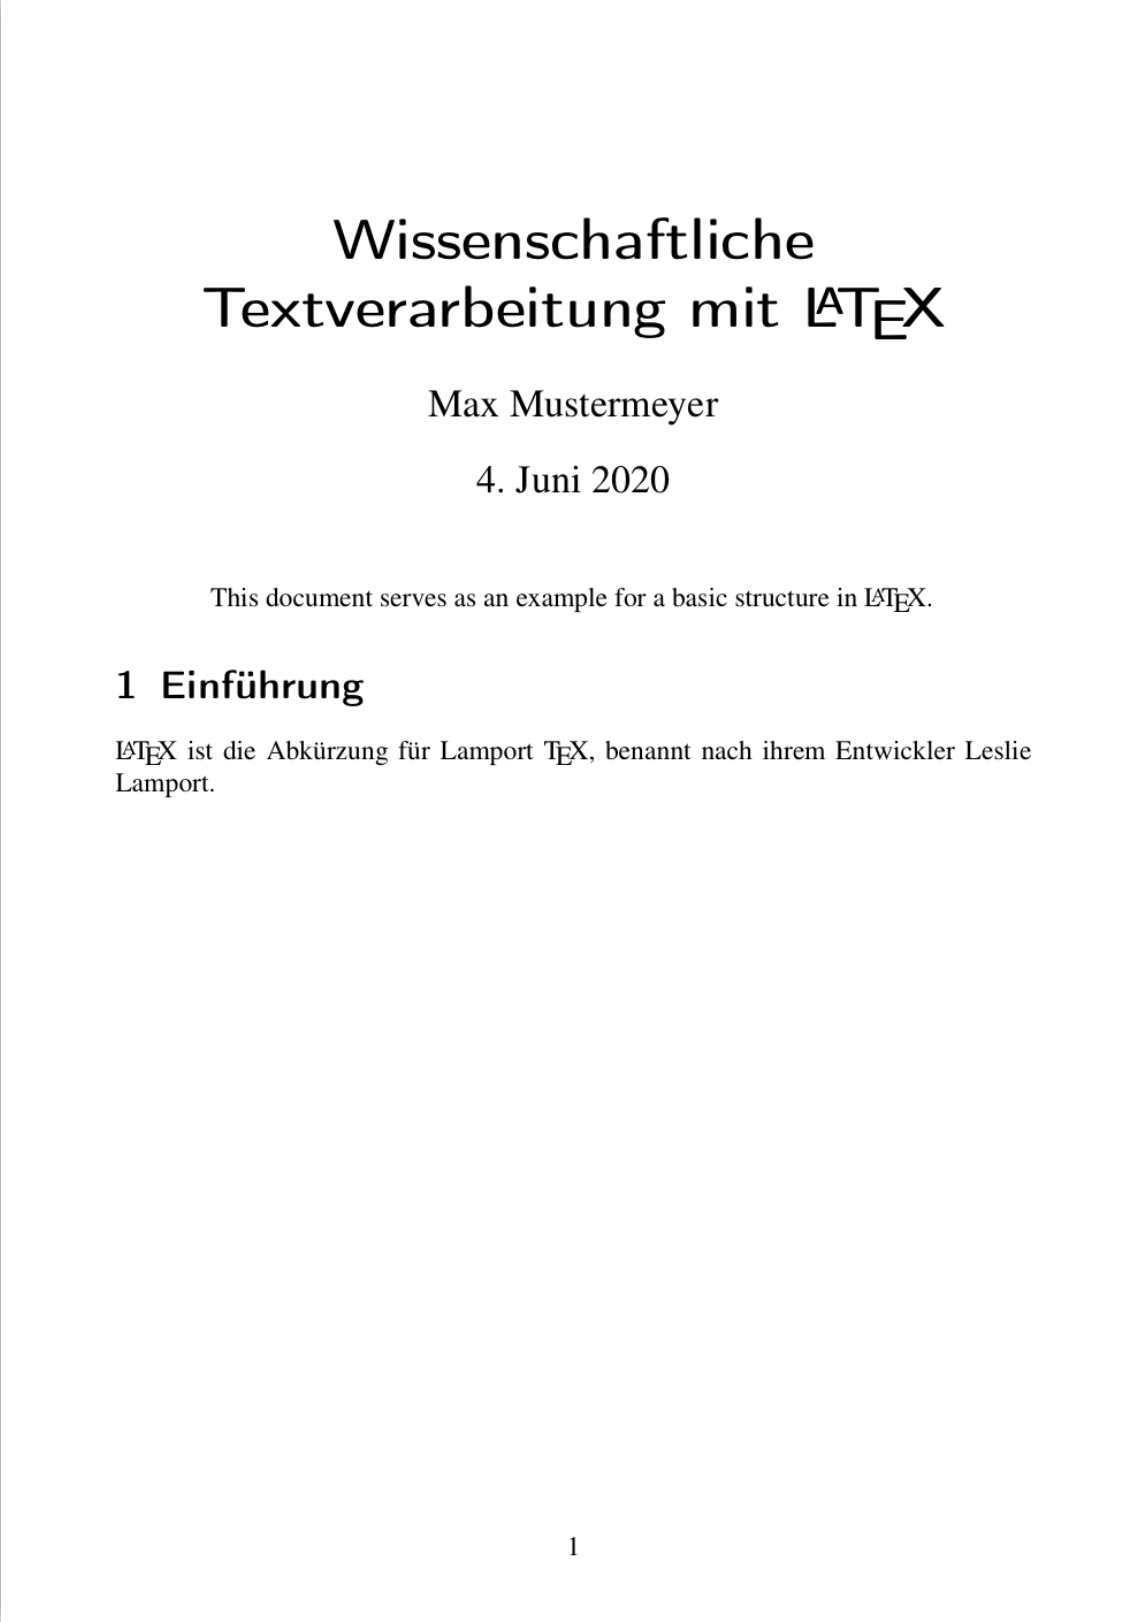
\includegraphics[scale=0.6]{graphics/ex1.png}}
    \caption[Dokumentenstruktur]{Beispielstruktur eines Dokuments}
    \label{fig:dokumentenstruktur}
\end{figure}

\subsection{Packages}
Die von der Dokumentenklasse definierten Standardeinstellungen und Funktionalitäten können mithilfe von Packages verändert und erweitert werden.
\begin{verbatim}
\usepackage{Paketname}
\end{verbatim}
Es gibt eine Vielzahl von Packages um das Dokument mit verschiedenen wünschnswerten Funktionen zu erweitern.
Packages können andere abhängige Packages laden.
Das Package lucida-utf lädt z.B. selbst das Package unicode-math, dieses lädt wiederum automatisch fontspec. \cite[vgl.][S.91ff]{Lamport1994}\\
Folgender Link bietet einen Katalog nützlicher verwendbarer Pakete: \\
\url{https://ctan.org/pkg}

\subsubsection{Schriften}
Die Verwendung einer Schriftart erfolgt über das einbinden des jeweiligen Schriftpakets.
\begin{verbatim}
\usepackage{Schriftpaketname}
\end{verbatim}
Ein offizieller Katalog kompatibler Schriften mit zugehörigen Schriftpaketen ist zu finden unter:\\ \url{https://tug.org/FontCatalogue/}\\\\
\paragraph{Wissenschaftliche Arbeit}In der Regel verwendet man in einer Wissenschaftlichen Arbeit eine Kombination aus drei verschiedenen Schriftfamilien: Roman(mit Serifen), Sans Serif(ohne Serifen) und Monospace. Es existieren nur wenige Schriftpakete, die eine komplette Definition dieser Schriftfamilien umfassen. Standardmäßig wird in \LaTeX\ eine Serifenschrift verwendet. Die verwendete Schriftfamilie lässt sich aber mit einzelnen Befehlen umschalten. In der folgenden Abbildung \ref{fig:schriften} kann man mehrere Schriftarten sehen. Der dazugehörige Code befindet sich in Listing \ref{lst:schriften}.\\\\
\begin{figure}[H]
    \centering
    
\includegraphics[scale=0.3]{graphics/schrift1.png}
    \caption[Schriften]{Verschiedene Schriftarten}
    \label{fig:schriften}
\end{figure}
Text kann \textbf{dick} \textit{kursiv} oder auch \underline{unterstrichen} sein.
\begin{listing}[H]
    \caption[Schriften]{Verwendung von Schriften in \LaTeX\ }
    \begin{minted}
    [
    firstnumber=1,
    frame=lines,
    framesep=2mm,
    baselinestretch=1.2,
    linenos
    ]
{Tex} 
\usepackage{mathptmx} % Schriftart: Times
\usepackage[scaled]{helvet}
\usepackage{courier}
\begin{document} 
\section{Beispiel}
Dieser Text ist normaler Text und deshalb in Times.\\
\textsf{Dieser Text ist serifenfreier Text und deshalb in Helvetica.}\\
\texttt{Dieser Text ist in Maschienenschrift und deshalb in Courier.}\\
\end{document}
    \end{minted}
    \label{lst:schriften}
\end{listing}
\pagebreak

\subsection{Listen}
Für Listen stehen grundsätzliich drei verschiedene Umgebungen zur Verfügung. Innerhalb der Umgebungen werden mit \texttt{\textbackslash item} die enthaltenen Punkte definiert. In dem folgenden Listing \ref{lst:listen} werden 2 Umgebungen gezeigt.\\
\noindent
\hspace*{\fill}
\begin{minipage}[t]{0.458\linewidth}
\centering
\vspace{0pt}
\begin{listing}[H]
    \caption[Listen]{Listen in \LaTeX\ }
    \begin{minted}
    [
    firstnumber=1,
    frame=lines,
    framesep=2mm,
    baselinestretch=1.2,
    linenos
    ]
{Tex} 
Itemize: 
\begin{itemize}[]
    \item Lachs
    \item Ingwer
    \item Öl
\end{itemize}
Enumerate: 
\begin{enumerate}[]
    \item Uno
    \item Dos
    \item Tres
\end{enumerate}
    \end{minted}
    \label{lst:listen}
\end{listing}
\end{minipage}
\hfill
\begin{minipage}[t]{0.5\linewidth}
\vspace{32pt}

Itemize: 
\begin{itemize}
    \item Lachs
    \item Ingwer
    \item Öl
\end{itemize}

Enumerate: 
\begin{enumerate}
    \item Uno
    \item Dos
    \item Tres
\end{enumerate}
\clearpage
\end{minipage}\\\\
Die verschidenen Umgebungen können auch miteinander verschachtelt werden. Das Paket \texttt{enumitem} ermöglicht die individuelle Bestimmung der Abstandgröße der Items einer Liste über die Variable \texttt{itemsep}. \cite[vgl.][S.24f]{Lamport1994}

